\documentclass[11pt, a4paper]{article}
\usepackage[slantfont, boldfont]{xeCJK}
\usepackage{ulem}
\usepackage{amsmath}
\usepackage{booktabs}
\usepackage{colortbl}
\usepackage{indentfirst}
\usepackage[top = 1.0in, bottom = 1.0in, left = 1.0in, right = 1.0in]{geometry}

\setCJKmainfont{SimSun}
\setCJKmonofont{SimSun}

\setlength{\parskip}{0.8\baselineskip}
\setlength{\parindent}{2em}

\newcolumntype{Y}{>{\columncolor{red}}p{12pt}}
\newcolumntype{N}{>{\columncolor{white}}p{12pt}}


\title{某AFO狗のNOI模拟题}
\author{by jiry\_2}


\begin{document}
\maketitle

\begin{center}
\emph{竞赛时长:5小时}
\end{center}
\begin{center}
\begin{tabular}{|l|p{70pt}|p{70pt}|p{70pt}|}
	\hline
	题目名称 & 数 & 树 & 数据结构\\
	\hline
	输入文件名 & number.in & tree.in & data.in \\
	\hline
	输出文件名 & number.out & tree.out & data.out \\
	\hline
	每个测试点时限 & $1$s & $1.5$s & $2.5$s\\
	\hline
	测试点数目 & $10$ & $10$ & $10$\\
	\hline
	每个测试点分值 & $10$ & $10$ & $10$\\
	\hline
	内存限制 & $512$MB & $512$MB & $512$MB\\
	\hline
	是否有部分分 & 否 & 否 & 否\\
	\hline
	题目类型 & 传统 & 传统 & 传统\\
	\hline
	是否有SPJ & 否&否 &否 \\
     \hline
\end{tabular}

测试时三题均开启 O2 优化开关。

\end{center}
\begin{center}
\end{center}

\newpage
\section{数}

\subsection{题目描述}
众所周知,萌萌哒六花不擅长数学,所以勇太给了她一些数学问题做练习,其中有一道是这样的:

一个正整数被称为是好的当且仅当它的十进制表示是其二进制表示的后缀。

例如正整数 $(100)_{10}$ 就是一个好的正整数,它的二进制表示是 $(1100100)_2$,而正整数 $(2)_{10}$ 就不是一个好的正整数,它的二进制表示是 $(10)_2$。

现在勇太想要知道第 $K$ 小的好的正整数。

当然,这个问题对于萌萌哒六花来说实在是太难了,你可以帮帮她吗?
\subsection{输入格式}
第一行输入一个正整数 $K$。
\subsection{输出格式}
输出一个整数表示答案。

\subsection{样例输入}
\begin{verbatim}
30
\end{verbatim}
\subsection{样例输出}
\begin{verbatim}
1010000
\end{verbatim}

\subsection{数据范围与约定}

对于 $10\%$ 的数据,$K \leq 40$。

对于 $30\%$ 的数据,$K \leq 300$。

对于 $50\%$ 的数据,$K \leq 800$。

对于 $70\%$ 的数据,$K \leq 7000$。

对于 $100\%$ 的数据,$K \leq 500000$。
\newpage
\section{串}

\subsection{题目描述}
众所周知,萌萌哒六花不擅长数学,所以勇太给了她一些数学问题做练习,其中有一道是这样的:

对于一张无向图,独立集定义为图的一个点集 $S$ 满足 $S$ 中任意两点之间都不存在一条边。定义一棵树的权值为这棵树的最大独立集大小。

现在勇太想要知道节点数 $a \in [1,n]$,权值 $b \in [0,n]$ 的有根树分别有多少棵,答案可能很大,他只想知道对 $998244353$ 取模后的结果。

在这个问题中每一个节点的儿子视为有序且互不相同的,具体可以见样例解释。
 
当然,这个问题对于萌萌哒六花来说实在是太难了,你可以帮帮她吗?
\subsection{输入格式}
输入第一行包含一个整数 $n$。

\subsection{输出格式}
输出 $n$ 行每行 $n+1$ 个整数,第 $i$ 行第 $j$ 列表示 $i$ 个节点权值为 $j-1$ 的树的个数。

\subsection{样例输入}
\begin{verbatim}
4
\end{verbatim}
\subsection{样例输出}
\begin{verbatim}
0 1 0 0 0
0 1 0 0 0
0 0 2 0 0
0 0 3 2 0
\end{verbatim}

\subsection{样例解释}
$4$ 个点不同的树有 $5$ 棵,如下图所示。它们的权值分别为 $2,3,2,2,3$。
\begin{center}
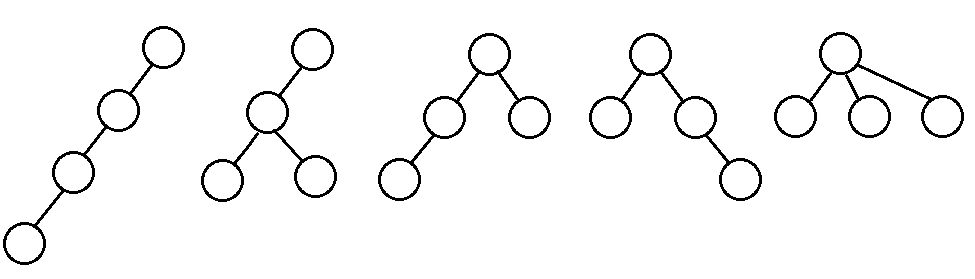
\includegraphics[width=0.9\linewidth]{2.png}
\end{center}
\subsection{数据范围与约定}

对于$10\%$的数据,$n \leq 15$。

对于$30\%$的数据,$n \leq 50$。

对于$60\%$的数据,$n \leq 200$。

对于$80\%$的数据,$n \leq 400$。

对于$100\%$的数据,$n \leq 500$。
\newpage
\section{数据结构}

\subsection{题目描述}
众所周知,萌萌哒六花不擅长数学,所以勇太给了她一些数学问题做练习,其中有一道是这样的:

定义一个数列的权值为它本质不同的子序列个数。例如数列 $(1,2,1)$ 的权值就是 $6$,它本质不同的子序列有 $(1),(2),(1,2),(2,1),(1,1),(1,2,1)$。 

给出一个长度为 $n$ 的数列 $A$ 和一个整数 $K$,保证 $A_i \in [0,K)$。接下来有 $m$ 次操作:

1. 给出 $l,r,x$,对所有的 $i \in [l,r]$,将 $A_i$ 变成 $(A_i+x) \mod K$。

2. 给出 $l,r,x$,对所有的 $i \in [l,r]$,将 $A_i$ 变成 $A_i \times x \mod K$。

3. 给出 $l,r$,询问区间 $[l,r]$ 的权值对 $998244353$ 取模后的值。
 
当然,这个问题对于萌萌哒六花来说实在是太难了,你可以帮帮她吗?
\subsection{输入格式}
第一行输入一个整数 $T$ 表示数组组数。

每组数据第一行输入三个整数 $n,K,m$。

第二行输入 $n$ 个整数表示数组 $A$。

接下来 $m$ 行每行第一个整数 $t$ 表示操作种类。

$t \in [1,2]$ 时接下来 $3$ 个整数 $l,r,x$,$t=3$ 时接下来两个整数 $l,r$。

\subsection{输出格式}
对于每个第三类操作输出一行一个整数表示答案。

\subsection{样例输入}
\begin{verbatim}
1
3 4 5
0 1 2
3 1 3
2 1 3 2
3 1 3
1 2 3 1
3 1 3
\end{verbatim}
\subsection{样例输出}
\begin{verbatim}
7
6
7
\end{verbatim}

\subsection{数据范围与约定}
对于 $10\%$ 的数据,$n \leq 20,m \leq 30$。

对于 $30\%$ 的数据,$n \leq 1000,m \leq 1000$。

对于 $50\%$ 的数据,$n \leq 10000,m \leq 10000$。

对于另外 $20\%$ 的数据,保证不存在第二类操作。

对于 $100\%$ 的数据,$n \leq 30000,m \leq 30000,K \leq 5, x\in [0,K),T \leq 2$。
\end{document}

